\documentclass[12pt,a4paper]{article}

\usepackage[left=0.6in,top=0.5in,right=0.6in,bottom=0.5in]{geometry}
\usepackage[T1]{fontenc}
\usepackage[utf8]{inputenc}
\usepackage{tikz}

\usetikzlibrary{positioning,fit,calc}

\setlength\parindent{0pt}
\newcommand{\tab}[1]{\hspace*{25pt}}
\tikzset{block/.style={draw, thick, text width=3cm, minimum height=1.5cm, align=center}, line/.style={-latex}}

\title{CS3152 Programming Languages Project Report}
\author{K. D. Sunera Avinash Chandrasiri (170081L)}

\begin{document}

\maketitle
\newpage

\section{Overall Structure}
    The structure of the program is divided mainly into 2 packages; \textbf{tree package} and \textbf{cse package}. Tree package functions will read the AST structure from the file and standardize the tree. Tree package will mainly rely on \textbf{Node} objects. Cse package functions will traverse the standardized tree structure and generate the control structures and evaluate the result. Similar to tree package, cse package will mainly rely on stacks of \textbf{Element} objects. \\


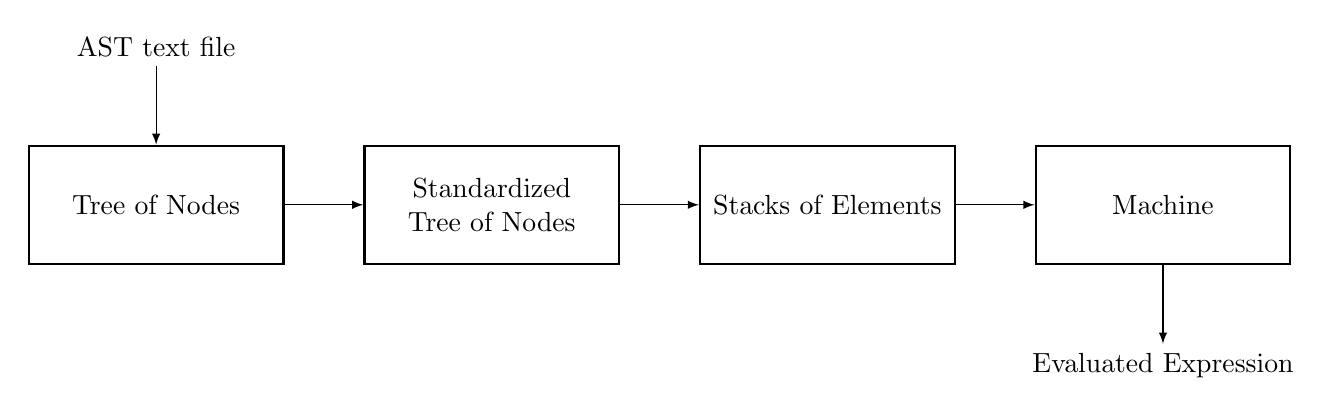
\begin{tikzpicture}
    \node                       (a) {AST text file};
    \node[block,below=of a]     (b) {Tree of Nodes};
    \node[block,right=of b]     (c) {Standardized Tree of Nodes};
    \node[block,right=of c]     (d) {Stacks of Elements};
    \node[block,right=of d]     (e) {Machine};
    \node[below=of e]           (f) {Evaluated Expression};

    \draw[line]               (a)-- (b);
    \draw[line]               (b)-- (c);
    \draw[line]               (c)-- (d);
    \draw[line]               (d)-- (e);
    \draw[line]               (e)-- (f);
\end{tikzpicture}

\section{Tree Package}
    This package will focus on reading the AST structure from the file and standardizing the tree. Following are the each class in this package and their objectives. \\

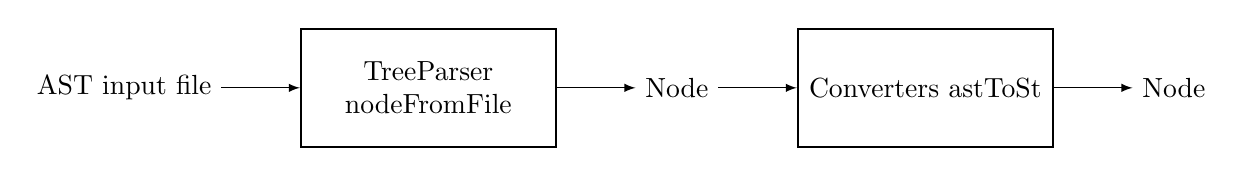
\begin{tikzpicture}
    \node                       (a) {AST input file};
    \node[block,right=of a]     (b) {TreeParser nodeFromFile};
    \node[right=of b]           (c) {Node};
    \node[block,right=of c]     (d) {Converters astToSt};
    \node[right=of d]           (e) {Node};

    \draw[line]               (a)-- (b);
    \draw[line]               (b)-- (c);
    \draw[line]               (c)-- (d);
    \draw[line]               (d)-- (e);
\end{tikzpicture}


\subsection{TreeParser class}
    Contains static utility functions to read the AST from file. \textit{nodeFromFile()} will read a \textit{Node} containing the AST structure from a given file. \\

    \begin{tabular}{lp{8cm}}
        \textbf{Node nodeFromFile(String fileName)} & Parse Node from the given file \\
        \textbf{Node nodeFromString(List<String> lines)} & Parse Node from a list of string lines \\
        \textbf{List<String> readFile(String fileName)} & Helper function to read a given file and output lines as an array of strings \\
        \textbf{String trimLeadingDots(String source)} & Helper function to trim leading dots from a string \\
        \textbf{String unescapeJavaString(String st)} & Helper function to unescape a string that contains standard escape sequences (\textbackslash n, \textbackslash t) \\
    \end{tabular}

\newpage

\subsection{Node class}
    Node will represent a tree node in the AST/ST structure. Following are the attributes of the Node;\\

    \begin{tabular}{lp{10cm}}
        \textbf{ArrayList<Node> children} & References to child nodes. \\
        \textbf{Node parent} & Reference to parent node (\textit{null} if this node is a root node). \\
        \textbf{String label} & Type of the node; let, where, lambda, id, str, int \\
        \textbf{String value} &  String representation of the value of the node(eg: string value of int node). This is not-null for leaf nodes.\\
    \end{tabular} \\

The class contains methods such as \textbf{copy()} method and methods to manipulate the tree structure such as \textbf{clearChildren()} and \textbf{addChild()}. \\

\subsection{Converters class}

A utility class to standardize the abstract syntax tree. \\

\begin{tabular}{lp{9cm}}
    \textbf{void astToSt(Node node)} & Converts the abstract syntax tree to a standardized tree recursively from the node. This uses below functions \\
    \textbf{void stForLet(Node rootNode)} & Standardize the LET node\\
    \textbf{void stForWhere(Node rootNode)} & Standardize the WHERE node\\
    \textbf{void stForFuncForm(Node rootNode)} & Standardize the FCN\_FORM node\\
    \textbf{void stForAnd(Node rootNode)} & Standardize the AND node\\
    \textbf{void stForRec(Node rootNode)} & Standardize the REC node\\
    \textbf{void stForLambda(Node rootNode)} & Standardize the Multi parameter function (lambda) node\\
    \textbf{void stForWithin(Node rootNode)} & Standardize the WITHIN node\\
    \textbf{void stForAt(Node rootNode)} & Standardize the @ node\\
\end{tabular} \\ \\

\subsection{Other classes}

\textbf{AstException} is a runtime exception which is thrown when standardizing the abstract syntax tree fails due to some reason.\\

\textbf{NodeWithDepth} is a Node class extended with depth attribute to help in reading the AST structure from the input file.\\

\section{CSE Package}

This package will traverse the standardized tree
structure and generate the control structures and evaluate the result.\\

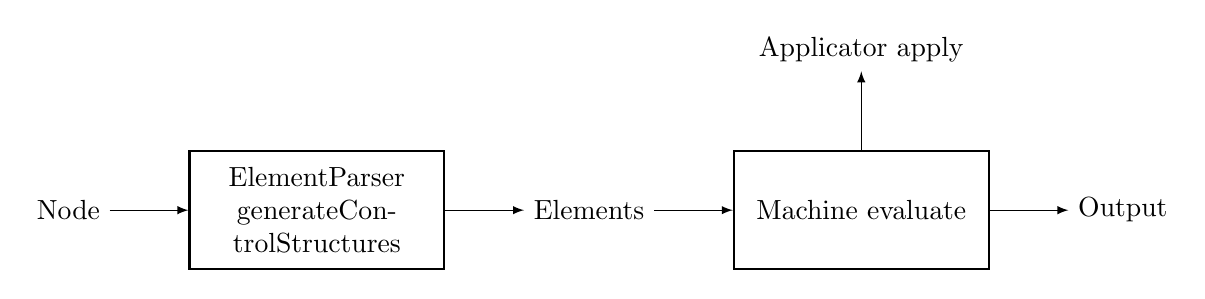
\begin{tikzpicture}
    \node                       (a) {Node};
    \node[block,right=of a]     (b) {ElementParser generateControlStructures};
    \node[right=of b]           (c) {Elements};
    \node[block,right=of c]     (d) {Machine evaluate};
    \node[above=of d]           (f) {Applicator apply};
    \node[right=of d]           (e) {Output};

    \draw[line]               (a)-- (b);
    \draw[line]               (b)-- (c);
    \draw[line]               (c)-- (d);
    \draw[line]               (d)-- (e);
    \draw[line]               (d)-- (f);
\end{tikzpicture} \\

\newpage
\subsection{ElementParser class}

This is a parser that will convert AST to Element stacks by pre-order traversal. This will create control structures; stacks of \textit{Value}.\\

\begin{tabular}{lp{9cm}}
    \textbf{generateControlStructures(Node root)} &  Generates the control structure array by pre-order traversal\\
    \textbf{generateCsForLambda(node, controls, ...)} & Split the control structure on \textit{lambda} nodes and use a \textit{delta} node to traverse in the sub tree \\
    \textbf{generateCsForIf(node, controls, ...)} & Split \textit{if} node to \textit{then} and \textit{else} delta nodes and traverse in sub-trees \\
    \textbf{generateCsForTau(node, controls, ...)} & Add number of elements in tau node and traverse in each sub-tree\\
\end{tabular} \\ \\

\subsection{Element package}

\subsubsection{Element abstract class}

Super element class which holds a \textbf{label} string. Label represents the type of the element such as lambda, delta.

\subsubsection{Value subclass}

This is the type of all elements except tuples. These have an additional \textbf{value} attribute of type \textbf{String} holding a string representation of the value stored inside the element. Value is null for types like \textit{true}, \textit{false}, \textit{id} and not-null for types like \textit{int}, \textit{str}.

\subsubsection{Tuple subclass}

This is the element of tuple type which can hold multiple elements. The \textbf{value} attribute of this subclass is of \textbf{Element[]} type which allows to hold child elements. The label of this element is \textit{tuple}.\\

\subsection{Environment class}

This is a class to represent the environment tree of the cse machine. Each environment has following attributes/methods. \\

    \begin{tabular}{lp{9cm}}
        \textbf{Environment parent} & Parent environment. Null if this is the primary environment. \\
        \textbf{HashMap<String, Element> memory} & Memory to hold values of each reference. In the primary environment, this will hold all the in-built function names. In other environments, memory will be initialized as empty. \\
        \textbf{void remember(String key, Element value)} & Remember an entry. This throws a runtime error if the key is already defined. \\
        \textbf{Element lookup(String id)} &  Get the value of a variable identified by the \textit{key}. Returns null if this is refers to an in-built value. If undefined, this throws a runtime error.\\
    \end{tabular} \\

\newpage

\subsection{Applicator package}

\subsubsection{Applicator class}

The utility class to apply in-built operators and functions to parameters. All the function applications will will be handled by the \textbf{apply} methods.
Following are the apply functions for unary functions and operators such as \textit{neg}, \textit{not} and binary operators such as \textit{+}, \textit{eq}. Also there are public helper functions to determine if an element is a binary operator or unary operator.\\

    \begin{tabular}{l}
        \textbf{Element apply(Element operation, Element operand)} \\
        \textbf{Element apply(Element operation, Element operand1, Element operand2)} \\
        \textbf{boolean isBinaryOperation(Element op)} \\
        \textbf{boolean isUnaryOperation(Element op)} \\
    \end{tabular} \\

Apart from that, there are other functions to perform the operator functionalities. \\

    \begin{tabular}{lp{6cm}}
        \textbf{numericalOperator(operand1, operand2, operation)} & Numeric operators helper \\
        \textbf{binaryBooleanOperator(operand1, operand2, operation)} & Boolean operators helper \\
        \textbf{covertToString(element)} & Element into string\\
        \textbf{booleanCondition(condition)} & Boolean primitive into element \\
        \textbf{substringOperation(operand, operation)} & String \textit{stem, stern} helper\\ \\
        \textbf{add(operand1, operand2)} & Addition operator \\
        \textbf{subtract(operand1, operand2)} & Subtraction operator \\
        \textbf{multiply(operand1, operand2)} & Multiplication operator \\
        \textbf{power( operand1, operand2)} & Power operator \\
        \textbf{divide(operand1, operand2)} & Division operator \\
        \textbf{print(operand)} & Print function \\
        \textbf{isString(operand)} & Check if string \\
        \textbf{isInteger(operand)} & Check if integer \\
        \textbf{isTruthValue(operand)} & Check if true/false \\
        \textbf{isTuple(operand)} & Check if tuple \\
        \textbf{order(operand)} & Length of tuple \\
        \textbf{stern(operand)} & String without first character \\
        \textbf{stem(operand)} & First character \\
        \textbf{conc(operand)} & String concatenation (partial) \\
        \textbf{conc(operator, operand2)} & String concatenation \\
        \textbf{iToS(operand)} & Integer to string \\
        \textbf{neg(operand)} & Negative value \\
        \textbf{or(operand)} & Or operator \\
        \textbf{and(operand)} & And operator \\
        \textbf{eq(operand)} & Equal operator \\
        \textbf{ne(operand)} & Not equal operator \\
        \textbf{gr(operand)} & Greater than operator \\
        \textbf{ls(operand)} & Less than operator \\
        \textbf{ge(operand)} & Greater than or equal operator \\
        \textbf{le(operand)} & Less than or equal operator \\
        \textbf{aug(operand1, operand2)} & Append element to tuple \\
        \textbf{extract(operation, operand)} & Extract element from tuple \\
    \end{tabular} \\

\subsubsection{Operation Interfaces definitions}

    \begin{tabular}{ll}
        \textbf{BinaryBooleanOperator} & Helper lambda closure of $(boolean, boolean) \rightarrow boolean$ \\
        \textbf{NumericalOperator} & Helper lambda closure of $(int, int) \rightarrow int$ \\
        \textbf{SubstringOperation} & Helper lambda closure of $(String) \rightarrow String$ \\
    \end{tabular} \\

\subsection{Machine class}

Machine class evaluates the control stack. Following are the main attributes.

\begin{tabular}{ll}
        \textbf{Stack<Value> control} & Control \\
        \textbf{Stack<Element> stack} & Stack \\
        \textbf{Applicator applicator} & Application controller \\
        \textbf{ArrayList<Environment> environments}&Environment array \\
        \textbf{ArrayList<Stack<Value> > controlStructures} & All control structures \\
        \textbf{void evaluate()} & Evaluate function to evaluate the stack control. \\
\end{tabular} \\

\textbf{evaluate()} will evaluate the control stack and apply CSE riles until control is empty.

\subsection{Other classes}

\textbf{CseException} is a runtime exception which is thrown when evaluating CSE machine fails due to some reason.\\

\textbf{Stack} Stack implementation to store Elements.\\

\end{document}

